\documentclass[../thesis.tex]{subfiles}
\renewcommand{\baselinestretch}{1.5}\selectfont
\graphicspath{{figs/}}
\begin{document}
\begin{refsection}
\chapter{Measurement Uncertainty}
\section{Introduction}

A measurement is an observation of a physical effect or quantity which provides useful information. This information, through the ages, has been used to facilitate advancement of both scientific knowledge and industrial development - from the production of standardised stone blocks to build the pyramids of ancient Egypt, to the production of standardised car parts to build Henry Ford's Model T. In the scientific realm, advanced measurement techniques at laboratories such as CERN are used to convince the world that new subatomic particles exist.

To communicate information about a measurement, the recipient needs to be able to either make or imagine a similar observation to that of the original measurer (or metrologist). The simplest way of doing this is to provide the recipient with the same physical effect or quantity for which to make their own observation (if you require a new nut for a bolt from a hardware shop, you might intuitively take the bolt with you), however, this can be inconvenient or impractical with larger objects, or if the recipient is located far away. Instead, you might substitute the physical effect or quantity with a more portable representation. For example, if you were to measure the size of a doorway to see if a new piece of furniture may fit through it, you might cut a piece of string to the same length and use this as the representation of the width of the item. However, this approach is very wasteful and also impractical for many physical effects (temperature, flow, pressure).

A solution widely thought to have been first established in the 3rd or 4th Millennium BC (see Figure 3.1), is a system of units. In such a system, a discretised value of a quantity is standardised and knowledge of its value is disseminated to all people who wish to use it. Typically, a range of discrete values are chosen, such that the system of units can be conveniently used to represent all measurements. Knowledge of the discretised values is obtained from a primary standard which becomes the definition of the unit and is used to create copies of the standard which can be given to users of the unit system to perform measurements with. The most common method of performing measurements with a unit system is to use a standard to calibrate a measuring instrument, which can then be used to measure an arbitrary value of a quantity in the units defined by the standard.

\begin{figure}
	\centering
	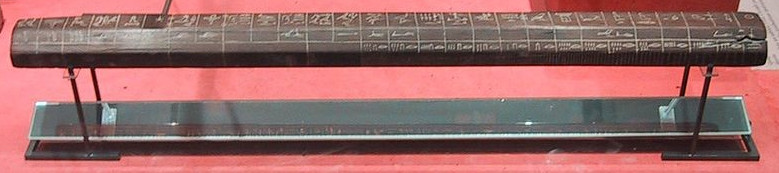
\includegraphics[width=\textwidth]{cubit}
	\caption{Egyptian royal cubit rod of Maya (treasurer of King Tutankhamun) 1336--1327 BC. The cubit is thought to be the earliest attested standard measure of length, first used in the 3rd or 4th Millennium BC.}
	\label{ch3_cubit}
\end{figure}

The introduction of a regulated system of units enables commerce, as traded goods can be reliably valued between merchants across cities. This application is encountered by all citizens, and so there is a high demand for standards to be produced from the primary standard and physically distributed. It becomes impractical to create all standards by copying the primary standard directly (in some cases because the value of the primary standard is perturbed each time it is measured), and so a tiered organisational structure of standards is used. In this structure, there is a tier consisting of a small number of standards which are created directly from measurements of the primary standard, followed by subsequent tiers of larger numbers of standards which are derived from measurements of those in the previous tier. For any standard produced, it should be possible to trace the lineage back to a measurement of the primary standard. This is referred to as a traceability chain (see Figure 3.2) and it is a fundamental tenet of metrology. Measurements with a shorter traceability chain are considered more traceable than those with longer chains.

Today, the primary standards are maintained in most countries by a National Measurement Institute (NMI) and co-ordinated by the Bureau of International Weights and Measures (BIPM). To accommodate international trade and compatibility, a routine process of inter-comparisons is undertaken to ensure that the values of the primary standards between countries are in agreement.

Secondary standards are also kept by the NMIs and are used to reduce excessive wear to the primary standard caused by frequent measurements (and also to reduce bottlenecks caused by having a single standard). They are calibrated against the primary standard as infrequently as possible, again to reduce wear. Secondary standards are used by the NMI to characterise working standards which are sent to them by manufacturers and research institutes. Another important task of each NMI is to perform investigations to discover new and improved methods of measurement, which make use of secondary standards to better compare the accuracy of different methods.

Working standards are used, for example, by instrumentation manufacturers who may use them to calibrate their products before shipping to the customer, and more generally the standards can be used to calibrate test equipment to identify faulty products. Larger research institutes typically use working standards to recalibrate instrumentation prior to performing very sensitive measurements. To ensure that product specifications and scientific measurements are traceable and of high quality, accreditation services such as the United Kingdom Accreditation Service (UKAS) exist to certify manufacturers and laboratories that demonstrate good measurement practice and use traceable measurements [2].

The selection of quantities for which primary standards are kept is only a subset of those for which recognised units exist. This is because many units are derived quantities, where their value can be obtained by calculation using definitions of other units. For example, the definition of the unit of resistance (R, ohms) can be derived from that of voltage (V, volts) and current (I, amperes), because R=V/I. The eight fundamental ``base'' units which make up the International System of Units (SI), are the metre, kilogram, second, ampere, kelvin, candela and mole. From these unit definitions, it is possible to define any other derived unit in use. NMIs will usually keep secondary standards of most derived quantities that users may wish to calibrate against, which are traceable to one or more primary standards of the base units. Although traditionally all primary standards were defined by physical artefacts (e.g. metallic weights, burning candles), these are being gradually replaced by definitions involving physical constants (e.g. Plank, Boltzmann), which do not degrade over time or use. The ``Ninth SI Units'' [3], a proposition recently accepted by the BIPM, covers the redefinition of four of the SI units (the ampere, the kilogram, the kelvin and the mole) which will come into effect by May 2019.

The crucial effect of traceability on measurements is the confidence in their results. Measurements with poor traceability (longer chains) will produce results which are likely to be less accurate than those with better traceability (shorter chains). The reason for this is measurement uncertainty, which will now be explained.

It is impossible to know the true value of a quantity being measured as many undesirable physical effects typically occur during the measurement process. These effects contribute error (an unwanted perturbation) to the measured value, causing a reduction in accuracy (the deviation of the  measured value from the true value). Typical sources of error in measurement include thermal noise, imperfect calibration and drift of environmental conditions from those at which a measuring instrument was calibrated. In some cases, it is possible to quantify and correct for these errors, but there are often many sources (some of which contribute very small errors) which cannot be corrected for. This is because either the error cannot be quantified or the value of the error will change over the duration of the measurement process (random errors). Any source of error which cannot be removed from a measurement becomes a source of uncertainty, because the deviation of the measured value from the true value due to this source of error is uncertain. If it is possible to quantify the amount of uncertainty in a measurement, then a degree of confidence can be formed about its value.
If every measurement has an associated uncertainty in its value, then any measurement involving the results of previous measurements will include uncertainty contributions from both measurements. Measurements with good traceability involve fewer sources of uncertainty than those with poor traceability, leading to a higher degree of confidence in the former. It is because of this fact that NMIs strive to reduce the uncertainties in their primary standard definitions, which in turn reduces the uncertainty in all traceable measurements.

Because it is impossible to know the amount of error in a source of uncertainty, probability and statistical theories are used to instead describe the amount of uncertainty associated with it. By the nature of these theories there are often several methods which can be used to obtain a result, which sometimes provide different values. To ensure consistency and portability of uncertainty definitions, measurement guides were created in each industry and area of science, which specialised in processing the results of typical measurements. In addition, different guides were produced depending on the level of accuracy required - as more accurate measurements often require more effort to complete. Although this practice allowed suitable measurement comparisons within each field (e.g. chemistry, mechanical engineering), ambiguities still existed in uncertainty definitions between fields. To address this, a landmark document was published in 1993 by the International Organisation for Standardisation (ISO), the Guide to the Expression of Uncertainty in Measurement (GUM) [4]. This document was the work of representatives from seven international organisations: the BIPM, the International Organisation of Legal Metrology (OIML), the International Electrotechnical Commission (IEC), the ISO, the International Federation of Clinical Chemistry and Laboratory Medicine (IFCC), the International Union of Pure and Applied Chemistry (IUPAC), and the International Union of Pure and Applied Physics (IUPAP). The GUM, updated in 2008 [5], is still used today as a reference for the evaluation of measurement uncertainty in many laboratories and industries across the world. The seven original organisations which wrote the GUM, together with the International Laboratory Accreditation Cooperation (ILAC, of which UKAS is a member), form the Joint Committee for Guides in Metrology (JCGM), who maintain the GUM and subsequent additional documents. These additional documents consist of the International Vocabulary of Metrology (VIM) [6] and two supplements to the GUM [7,8]: Supplement 1 covers the use of a Monte Carlo method [9] in uncertainty evaluation; Supplement 2 is used where more than one quantity is measured at the same time (multivariate).
Throughout this dissertation, the methodologies presented in the GUM will be used. The international authority of the guide, developed by seven international organisations (including the two global standardisation bodies IEC and ISO), gives strong motivation to use it as a basis for a framework to evaluate uncertainty in measurement.
This Chapter describes the evaluation of uncertainty prescribed in the GUM and highlights an inconsistency in the current version of the GUM and associated documents (which can have a profound effect on electromagnetic measurements).

\section{The Measurement Process}

In contrast to basic evaluations of uncertainty, where only repeat measurements of the quantity of interest are analysed, the GUM prescribes a more rigorous approach, which defines a mathematical model of the measurement process (measurement model) and propagates uncertainty through that model to the result (measurands). This allows any uncertainties from previous measurements, including those involving standards in the traceability chain, to be included in the result. The measurement model can be simple, such as measuring resistance using input quantities of voltage and current, or complicated and multivariate, requiring many input quantities and producing many output quantities. In some cases, the measurement model may not be known and can be defined as a black box, but this has certain limitations discussed later with Monte Carlo methods.

The GUM defines a process that is to be followed when evaluating uncertainty in measurement. It consists of the following steps:

\begin{enumerate}
	\item Modelling the measurement.
	\item Evaluating standard uncertainty of input quantities.
	\item Determining combined standard uncertainty of the measurands.
	\item Determining expanded uncertainty of the measurands.
\end{enumerate}

where standard uncertainty is an uncertainty expressed as a standard deviation and expanded uncertainty defines an interval encompassing a large fraction of the distribution of values that could reasonably be attributed to the measurand.

\subsection{Modelling the Measurement}

\subsection{Evaluating Standard Uncertainty of Input Quantities}

\subsubsection{Category A Evaluation}
\subsubsection{Category B Evaluation}
\subsection{Evaluating Combined Standard Uncertainty}
\subsubsection{Monte Carlo Methods}
\subsubsection{Law of Propagation of Uncertainty}
\subsubsection{Finite Difference Methods}
\subsection{Expanded Uncertainty and Coverage Intervals}
\section{Sensitivity Analysis}
\section{Conclusions}
Testing, testing2\cite{Stant_2017}.
\addcontentsline{toc}{section}{Bibliography}
\printbibliography
\end{refsection}
\end{document}
